% Options for packages loaded elsewhere
\PassOptionsToPackage{unicode}{hyperref}
\PassOptionsToPackage{hyphens}{url}
%
\documentclass[
]{article}
\usepackage{amsmath,amssymb}
\usepackage{iftex}
\ifPDFTeX
  \usepackage[T1]{fontenc}
  \usepackage[utf8]{inputenc}
  \usepackage{textcomp} % provide euro and other symbols
\else % if luatex or xetex
  \usepackage{unicode-math} % this also loads fontspec
  \defaultfontfeatures{Scale=MatchLowercase}
  \defaultfontfeatures[\rmfamily]{Ligatures=TeX,Scale=1}
\fi
\usepackage{lmodern}
\ifPDFTeX\else
  % xetex/luatex font selection
\fi
% Explicit Unicode mapping for the pandoc-generated body under pdflatex
% (utf8 inputenc does not define Greek / math symbols by default).
\ifPDFTeX
\usepackage{newunicodechar}
\newunicodechar{Λ}{\ensuremath{\Lambda}}
\newunicodechar{Σ}{\ensuremath{\Sigma}}
\newunicodechar{Φ}{\ensuremath{\Phi}}
\newunicodechar{β}{\ensuremath{\beta}}
\newunicodechar{λ}{\ensuremath{\lambda}}
\newunicodechar{μ}{\ensuremath{\mu}}
\newunicodechar{ρ}{\ensuremath{\rho}}
\newunicodechar{τ}{\ensuremath{\tau}}
\newunicodechar{—}{---}
\newunicodechar{−}{\textminus}
\newunicodechar{≅}{\ensuremath{\cong}}
\newunicodechar{≈}{\ensuremath{\approx}}
\newunicodechar{⊗}{\ensuremath{\otimes}}
\newunicodechar{⊗}{\ensuremath{\otimes}}
\newunicodechar{×}{\ensuremath{\times}}
\newunicodechar{Γ}{\ensuremath{\Gamma}}
\newunicodechar{→}{\ensuremath{\to}}
\newunicodechar{Δ}{\ensuremath{\Delta}}
\newunicodechar{Ĩ}{\ensuremath{\tilde{I}}}
\newunicodechar{§}{\S}
\newunicodechar{–}{--}
% Table support (pandoc longtable output)
\usepackage{longtable,booktabs,array}
\usepackage{calc}
\fi
% Use upquote if available, for straight quotes in verbatim environments
\IfFileExists{upquote.sty}{\usepackage{upquote}}{}
\IfFileExists{microtype.sty}{% use microtype if available
  \usepackage[]{microtype}
  \UseMicrotypeSet[protrusion]{basicmath} % disable protrusion for tt fonts
}{}
\makeatletter
\@ifundefined{KOMAClassName}{% if non-KOMA class
  \IfFileExists{parskip.sty}{%
    \usepackage{parskip}
  }{% else
    \setlength{\parindent}{0pt}
    \setlength{\parskip}{6pt plus 2pt minus 1pt}}
}{% if KOMA class
  \KOMAoptions{parskip=half}}
\makeatother
\usepackage{xcolor}
\setlength{\emergencystretch}{3em} % prevent overfull lines
\providecommand{\tightlist}{%
  \setlength{\itemsep}{0pt}\setlength{\parskip}{0pt}}
\setcounter{secnumdepth}{-\maxdimen} % remove section numbering
\ifLuaTeX
  \usepackage{selnolig}  % disable illegal ligatures
\fi
\usepackage{bookmark}
\IfFileExists{xurl.sty}{\usepackage{xurl}}{} % add URL line breaks if available
\urlstyle{same}
\hypersetup{
  hidelinks,
  pdfcreator={LaTeX via pandoc}}

\author{}
\date{}

\begin{document}

\section{Abstract}\label{abstract}

Variational tensor-product selection (TPS) over the unitary quotient
\(\mathcal{U}/\mathcal{U}_A \times \mathcal{U}_B\) is a candidate
mechanism for structural emergence in open quantum systems: given a
state \(\rho\) and a Liouvillian \(L\), a factorization
\(F^* = F^*(\rho, L, \lambda)\) is chosen by optimizing an objective
\(\Phi_F = I_F - \lambda J_F\) that balances the mutual information
articulated by the cut against its dynamical stability. We show that the
natural normalized decay-rate functional is \textbf{singular} on the
unrestricted quotient: the denominator \(|Q_F\rho|^2\) can vanish,
driving the objective to \(+\infty\) along non-physical near-product
directions. We replace it with the unnormalized functional
\(J_{\mathrm{dyn}}^{(0)} = -\mathrm{Re}
\langle Q_F\rho, Q_FL(\rho)\rangle\) and demonstrate numerically that
singularity, product collapse, and seed instability disappear. The
selected factorization responds systematically to both the Hamiltonian
and the state (cross-evaluation matrix diagonal dominance). Extending
the functional to a finite observation window \(\tau\) reveals
\textbf{competing structural basins}: the instantaneously optimal
factorization and a distinct finite-time-optimal factorization cross at
\(\Delta\Phi(\tau_c) = 0\), with
\(\tau_c = 0.0180, 0.0206, 0.0224, 0.0217\) for \(N = 3,4,4,5\) (cuts
\(2|1\), \(2|2\), \(1|3\), \(2|3\)) --- an essentially size-independent
finite-size trend. The crossover scale is \textbf{derived}, not fitted:
to first order in the finite-time expansion
\(\tau_c^{(1)} = -\Delta\Phi_0/\Delta\Phi_1\) reproduces the measured
values within 5--11\%, and the quadratic correction within 0.0--0.5\%.
The crossover timescale is therefore set by the objective balance
between competing structural basins, not by the global Liouvillian
relaxation time (\(\tau_c \Delta_L = 0.012\); the \(O(1)\) hypothesis is
rejected). The falsification-then-replacement arc is the central result:
a canonical functional was shown to be ill-posed mid-course, and its
replacement survived a battery of tests including a finite-size
persistence check.

\section{1. Introduction}\label{introduction}

Tensor-product structures (TPS) are the mathematical backbone of quantum
information: bipartite cuts, entanglement wedges, and decoherence-free
subspaces are all statements about which factorization of Hilbert space
\(\mathcal{H} \simeq \mathcal{H}_A \otimes \mathcal{H}_B\) captures the
physics. In the Relational Emergence Model (REM) the factorization is
not fixed a priori: it is a \textbf{selected structure} \(F^*\) obtained
by optimizing a variational objective over the unitary quotient
\(\mathcal{U}(d)/[\mathcal{U}(d_A)\times\mathcal{U}(d_B)]\), where
\(d = d_A d_B\) {[}Maruko, REM series; Spec v2.2{]}. The selection
depends on the state \(\rho\), the generator \(L\) of the open-system
dynamics, and the trade-off parameter \(\lambda\):

\[F^* = F^*(\rho, L, \lambda).\]

Two questions dominate the program. First, \textbf{which objective is
well-posed?} A naive candidate --- the normalized local decay rate
\(\Gamma_F = -\mathrm{Re}\langle Q_F\rho, Q_FL(\rho)\rangle/|Q_F\rho|^2\)
--- turns out to be singular on the unrestricted quotient (Claim 1). The
denominator measures how far the rotated state is from the TPS algebra;
on the quotient it can approach zero, so \(\Gamma_F\) diverges and the
optimizer escapes to non-physical near-product configurations. The
resolution is the denominator-free canonical functional

\[J_{\mathrm{dyn}}^{(0)}(F;\rho,L) = -\mathrm{Re}\langle Q_F\rho, Q_F
L(\rho)\rangle, \qquad \Phi_F = I_F - \lambda J_{\mathrm{dyn}}^{(0)},\]

which is bounded by Cauchy--Schwarz and vanishes smoothly in the
singular direction (Claim 2).

Second, \textbf{how does the selected structure depend on the
observation scale?} Extending \(J_{\mathrm{dyn}}^{(0)}\) to a finite
window \(J_{\mathrm{dyn}}^{(\tau)}\) exposes a genuinely new phenomenon:
for the maximally entangled (Haar) state the instantaneous optimum and
the finite-time optimum belong to \textbf{different structural basins},
and the two basins' objectives cross at a scale \(\tau_c \approx 0.02\)
(Claim 4a). The crossover persists at \(N=4,5\) with an essentially flat
\(\tau_c(N)\) (Claim 4b), and its scale is explained analytically by the
leading terms of the finite-time expansion (Claim 4c).

The paper is organized around four claims and their evidence, following
the chronology of the research: the falsification (Claim 1), the
well-posed replacement (Claim 2), the structural response (Claim 3), and
the finite-time crossover with its mechanism (Claims 4a--4c). All
numerical results are reproducible from the public repository (branch
\texttt{open}); the frozen specification is \texttt{REM\ Spec\ v2.2},
and this paper's numerical evidence is catalogued separately in the
\texttt{Spec\ v2.2\ Validation\ Addendum\ —\ Phase\ D\ Results} so that
theory specification and post-hoc evidence remain cleanly separated.

\section{2. Formalism}\label{formalism}

\subsection{2.1 System}\label{system}

We consider \(N\) qubits (\(N = 3,4,5\)), \(d = 2^N\), with a fixed
bipartition \(\mathcal{H} = \mathcal{H}_A \otimes \mathcal{H}_B\) of
dimensions \((d_A, d_B)\): \(2|1\) (\(N=3\)), \(2|2\) and \(1|3\)
(\(N=4\)), \(2|3\) (\(N=5\)). The Hamiltonian is an asymmetric XY chain

\[H = \sum_{i=1}^{N-1} J_i (X_i X_{i+1} + Y_i Y_{i+1}) + h \sum_i Z_i,\]

with \(J_1 = 1.5\), \(J_i = 0.6\) (\(i\ge 2\)), \(h = 0.2\). The
environment is pure dephasing with per-site rates
\(\gamma = (0.5, 1.0, 2.0)\) (periodically extended for \(N>3\)), giving
the Lindbladian

\[L(\rho) = -i[H,\rho] + \sum_i \frac{\gamma_i}{2}\big(2 Z_i \rho Z_i -
\rho Z_i^2 - Z_i^2 \rho\big).\]

States: the ground state of \(H\), a Haar (maximally entangled) pure
state, a mixed state, and a thermal state (see Sec. 5). All
optimizations use Adam (\(\mathrm{lr}=10^{-2}\)), \(6\) seeds for
\(N=3\) (\(4\) for \(N\ge4\)), and \(\lambda = 0.2\).

\subsection{2.2 Tensor-product structures and the canonical
functional}\label{tensor-product-structures-and-the-canonical-functional}

A TPS is an algebra
\(A_F = U\big(\mathcal{L}(\mathcal{H}_A)\otimes I_B\big)
U^\dagger\) generated by a unitary \(U\) on the quotient. Given the
dominant eigenvector \(\psi_U\) of \(U^\dagger \rho U\), the Schmidt
basis defines the projector \(Q_F\) onto the orthogonal complement of
\(A_F\) acting on operators (dephasing projection). The canonical
dynamical functional is

\[J_{\mathrm{dyn}}^{(0)}(F;\rho,L) = -\mathrm{Re}\langle Q_F\rho,
Q_F L(\rho)\rangle,\]

where \(\langle A,B\rangle = \mathrm{Tr}(A^\dagger B)\) is the
Hilbert--Schmidt inner product. By Cauchy--Schwarz,

\[|J_{\mathrm{dyn}}^{(0)}| \le |Q_F\rho|\,|Q_FL(\rho)|,\]

so \(J_{\mathrm{dyn}}^{(0)} \to 0\) smoothly as \(|Q_F\rho|^2 \to 0\);
there is no denominator to blow up. The variational objective is

\[\Phi(F;\lambda) = I_\rho(F) - \lambda J_{\mathrm{dyn}}^{(0)}(F),
\qquad [J] = T^{-1},\ [\lambda] = T,\]

with \(I_\rho(F)\) the mutual information across the cut of the rotated
state. The selected structure is \(F^* = \arg\max_F \Phi(F;\lambda)\).

\subsection{2.3 Finite-time extension}\label{finite-time-extension}

The operational extension measures the average decay of the residual
over a window \(\tau\):

\[J_{\mathrm{dyn}}^{(\tau)}(F) = -\frac{C_F^2(\tau) - C_F^2(0)}{2\tau},
\qquad C_F^2(t) = |Q_F\, U^\dagger e^{tL}\rho\, U|^2,\]

with \(Q_F\) fixed at the \(t=0\) Schmidt basis. The exact derivative
identity
\(dC_F^2/dt\big|_0 = 2\mathrm{Re}\langle Q_F\rho, Q_FL(\rho)\rangle\)
gives the consistency condition

\[\lim_{\tau\to 0} J_{\mathrm{dyn}}^{(\tau)} = J_{\mathrm{dyn}}^{(0)},\]

verified numerically to \(\le 2.5\times10^{-3}\) at \(\tau = 10^{-3}\).

\subsection{2.4 Crossover definition}\label{crossover-definition}

For a pair of competing basins with representatives \((F_A, F_B)\)
(fixed from independent optimizations at small and large \(\tau\)), the
objective difference

\[\Delta\Phi(\tau) = \Phi_\tau(F_B) - \Phi_\tau(F_A)\]

is evaluated at the \textbf{fixed} representatives. The crossover
timescale \(\tau_c\) is defined by the objective crossing
\(\Delta\Phi(\tau_c) = 0\) --- never by the optimizer's basin hops.

\section{3. Claim 1 --- the normalized functional is singular
(D2.1)}\label{claim-1-the-normalized-functional-is-singular-d2.1}

The pre-canonical candidate was the normalized local decay rate

\[\Gamma_F^{(0)} = -\frac{\mathrm{Re}\langle Q_F\rho, Q_FL(\rho)\rangle}
{|Q_F\rho|^2}.\]

\textbf{Claim 1.} \emph{On the unrestricted TPS quotient,
\(\Gamma_F^{(0)}\) is singular as a variational objective: the optimizer
drives \(|Q_F\rho|^2 \to 0\), which sends \(\Gamma_F \to \pm\infty\) and
\(\Phi \to +\infty\) along non-physical near-product directions.}

\emph{Evidence (Haar states, full quotient, \(N=3\)).} The optimizer
exploits the denominator directly:

\begin{itemize}
\tightlist
\item
  correlation of the objective with the log residual:
  \(\mathrm{corr}(\Phi, \log_{10} C_F^2(0)) = -0.999\);
\item
  the best trial reaches \(C_F^2(0) = 6\times10^{-4}\) with \(\Gamma \to
  -129\) and \(\Phi = 25.7\) (vs.~the well-behaved optimum
  \(\Phi \approx
  1.86\) under the unnormalized functional); the minimum residual across
  trials is \(C_F^2 = 4\times10^{-4}\);
\item
  the selected structure collapses toward a product state: the largest
  Schmidt \(p_{\max} = 0.9998\) among trials;
\item
  a singularity-direction sweep (approaching \(|Q_F\rho|^2 \to 0\)
  directly) confirms the blow-up.
\end{itemize}

Since every pure state can be approached by a product-state TPS, the
denominator can vanish on any open neighborhood of the quotient. The
normalized rate is therefore retained only as a \textbf{fixed-\((F)\)
local diagnostic} (Spec v2.2 §7) and is \textbf{prohibited as a global
variational objective}.

\begin{figure}
\centering
\pandocbounded{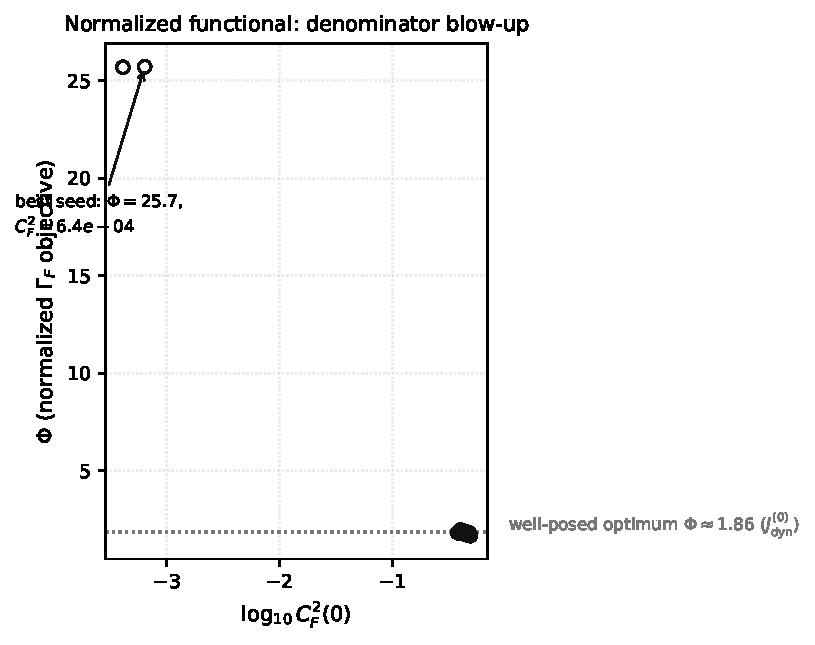
\includegraphics[keepaspectratio,alt={Figure 1: Normalized functional breakdown (Claim 1, D2.1). The variational objective \textbackslash Phi vs \textbackslash log\_\{10\} C\_F\^{}2(0) over 30 Haar seeds on the unrestricted quotient. \textbackslash mathrm\{corr\}(\textbackslash Phi,\textbackslash log\_\{10\} C\_F\^{}2(0)) \textbackslash approx
-0.999: as the denominator \textbar Q\_F\textbackslash rho\textbar\^{}2 \textbackslash to 4\textbackslash times10\^{}\{-4\} the objective blows up to \textbackslash Phi = 25.7 (best seed, annotated) and the Schmidt spectrum collapses toward a product state (p\_\{\textbackslash max\} = 0.9998). The dotted line marks the well-posed optimum \textbackslash Phi \textbackslash approx 1.86 under J\_\{\textbackslash mathrm\{dyn\}\}\^{}\{(0)\}.}]{figures/fig1_falsification}}
\caption{Figure 1: Normalized functional breakdown (Claim 1, D2.1). The
variational objective \(\Phi\) vs \(\log_{10} C_F^2(0)\) over 30 Haar
seeds on the unrestricted quotient.
\(\mathrm{corr}(\Phi,\log_{10} C_F^2(0)) \approx
-0.999\): as the denominator \(|Q_F\rho|^2 \to 4\times10^{-4}\) the
objective blows up to \(\Phi = 25.7\) (best seed, annotated) and the
Schmidt spectrum collapses toward a product state
(\(p_{\max} = 0.9998\)). The dotted line marks the well-posed optimum
\(\Phi \approx 1.86\) under \(J_{\mathrm{dyn}}^{(0)}\).}
\end{figure}

\section{4. Claim 2 --- the unnormalized functional is well-posed
(D2.2)}\label{claim-2-the-unnormalized-functional-is-well-posed-d2.2}

\textbf{Claim 2.} \emph{Under \(J_{\mathrm{dyn}}^{(0)}\), singularity,
product collapse, and seed instability disappear; the optimization is
well-posed on the unrestricted quotient.}

\emph{Evidence (D2.2-A; frozen D2 protocol, only the dynamical term
changed).}

{\def\LTcaptype{none} % do not increment counter
\begin{longtable}[]{@{}
  >{\raggedright\arraybackslash}p{(\linewidth - 6\tabcolsep) * \real{0.2500}}
  >{\raggedright\arraybackslash}p{(\linewidth - 6\tabcolsep) * \real{0.2500}}
  >{\raggedright\arraybackslash}p{(\linewidth - 6\tabcolsep) * \real{0.2500}}
  >{\raggedright\arraybackslash}p{(\linewidth - 6\tabcolsep) * \real{0.2500}}@{}}
\toprule\noalign{}
\begin{minipage}[b]{\linewidth}\raggedright
State
\end{minipage} & \begin{minipage}[b]{\linewidth}\raggedright
\(\Phi^*\) under \(\Gamma\) (superseded)
\end{minipage} & \begin{minipage}[b]{\linewidth}\raggedright
\(\Phi^*\) under \(J^{(0)}\)
\end{minipage} & \begin{minipage}[b]{\linewidth}\raggedright
seed std
\end{minipage} \\
\midrule\noalign{}
\endhead
\bottomrule\noalign{}
\endlastfoot
ground & 1.7993 & \textbf{1.8995} & 0.0007 \\
haar & 49.10 (singular) & \textbf{1.8594} & 0.0090 \\
mixed & 1.8485 & \textbf{1.9845} & 0.0051 \\
thermal & 1.8499 & \textbf{1.9465} & 0.0058 \\
\end{longtable}
}

\begin{itemize}
\tightlist
\item
  \textbf{No singularity}: minimum \(C_F^2(0) = 0.0956\) (vs
  \(4\times10^{-4}\) under \(\Gamma\)); maximum
  \(|\gamma_{\mathrm{ref}}| = 1.66\); the optimizer never approaches the
  singular region.
\item
  \textbf{No product collapse}: Schmidt \(p_{\max} \in [0.51, 0.58]\)
  (vs \(0.9997\) under \(\Gamma\)); the Haar state retains genuine
  multi-partite correlation (\(N=3\)).
\item
  \textbf{Seed stability}: 30-seed Haar run: best \(1.8595\), std
  \(0.0077\) (vs \(25.71 / 5.96\) under \(\Gamma\)); per-state std
  \(\le 0.009\).
\item
  \textbf{Continuity}: perturbation analysis gives \(\max|\Delta\Phi| =
  7.7\times10^{-5}\) across 9 independent quotient directions.
\item
  \textbf{Tradeoff}: \(\Phi = I - \lambda J\) retains the monotone
  \(\lambda\)-tradeoff (Spec v2.2 §5).
\end{itemize}

\emph{Consistency with the finite-time extension (D2.2-B).} The
derivative identity holds (\(\mathrm{dev} \approx 0.96\,\tau\,|J_0|\),
\(\le 2.5\times
10^{-3}\) at \(\tau=10^{-3}\)); all states share the same basin at
\(\tau \le 3\times10^{-3}\); the state ranking
\(\Phi_{\mathrm{mixed}} > \Phi_{\mathrm{thermal}} > \Phi_{\mathrm{ground}}
> \Phi_{\mathrm{haar}}\) is preserved at every \(\tau\); and no
pathology recurs on the window \(\tau \in [10^{-3}, 10^{-1}]\). The Haar
basin transition observed at larger \(\tau\) is the subject of Claim 4a.

\section{5. Claim 3 --- structural response (D1-R,
D2-R)}\label{claim-3-structural-response-d1-r-d2-r}

\textbf{Claim 3.} \emph{The selected structure responds to both the
Hamiltonian and the state: \(F^* = F^*(\rho, L, \lambda)\), not a
state-independent common solution.}

\emph{Hamiltonian response (D1-R; 5 families, 6 seeds each).}

{\def\LTcaptype{none} % do not increment counter
\begin{longtable}[]{@{}lll@{}}
\toprule\noalign{}
Family & \(\Phi^*\) & seed std \\
\midrule\noalign{}
\endhead
\bottomrule\noalign{}
\endlastfoot
asymmetric\_XY & 1.8994 & 0.0007 \\
transverse\_field\_ising & 1.8246 & 0.0010 \\
heisenberg\_xxz & 1.8695 & 0.0002 \\
xyz & 1.8740 & 0.0006 \\
random\_local & 1.8481 & 0.0007 \\
\end{longtable}
}

The cross-evaluation matrix \(\Phi_{H_i}(F^*_j)\) is diagonally
dominant: mean gap \(0.113\) (asym \(0.068\), ising \(0.092\),
heisenberg \(0.106\), xyz \(0.025\), random \(0.274\)). Geometrically,
physically related families are closer in the quotient
(\(d_F(\mathrm{asym},\mathrm{random}) = 0.412\),
\(d_F(\mathrm{ising},\mathrm{xyz}) = 0.559\); all others \(\approx
0.87\text{–}0.88\)).

\emph{State response (D2-R; 4 states, 6 seeds each, fixed
asymmetric\_XY).}

{\def\LTcaptype{none} % do not increment counter
\begin{longtable}[]{@{}lll@{}}
\toprule\noalign{}
State & \(\Phi^*\) & seed std \\
\midrule\noalign{}
\endhead
\bottomrule\noalign{}
\endlastfoot
ground & 1.8995 & 0.0007 \\
haar & 1.8594 & 0.0090 \\
mixed & 1.9845 & 0.0051 \\
thermal & 1.9465 & 0.0058 \\
\end{longtable}
}

Cross-evaluation matrix \(\Phi_{\rho_i}(F^*_j)\) (rows = state
objective, columns = \(F^*_j\) for ground, haar, mixed, thermal):

{\def\LTcaptype{none} % do not increment counter
\begin{longtable}[]{@{}lllll@{}}
\toprule\noalign{}
state ~\(F^*_j\) & ground & haar & mixed & thermal \\
\midrule\noalign{}
\endhead
\bottomrule\noalign{}
\endlastfoot
ground & 1.900 & 1.175 & 1.899 & 1.772 \\
haar & 1.528 & 1.859 & 1.328 & 1.288 \\
mixed & 1.926 & 1.198 & 1.985 & 1.806 \\
thermal & 1.416 & 1.611 & 1.699 & 1.947 \\
\end{longtable}
}

Mean gap \(0.159\) (ground \(0.000\), haar \(0.332\), mixed \(0.058\),
thermal \(0.247\)). Geometrically
\(d_F(\mathrm{ground},\mathrm{mixed}) = 0.343\) (close), while
\(d_F(\mathrm{mixed},\mathrm{thermal}) = 0.868\) despite similar
\(\Phi\) values --- closeness in objective does \textbf{not} imply the
same structure. Precise wording: \emph{state-dependent response is
established overall, although ground and mixed contain nearly degenerate
optima under the ground-state objective} --- the separation strength
varies by pair.

\section{6. Claim 4a --- finite-time structural crossover
(D3)}\label{claim-4a-finite-time-structural-crossover-d3}

\textbf{Claim 4a.} \emph{For the Haar state, the instantaneous optimum
and the finite-time optimum belong to distinct structural basins, and
their objectives cross at \(\tau_c = 0.0180\): the selected structure
depends on the dynamical observation scale.}

\emph{Method.} Representatives \(F_A\) (D2.2-A Haar optimum) and \(F_B\)
(\(\tau=0.1\) Haar optimum) are fixed once; \(\Delta\Phi(\tau) =
\Phi_\tau(F_B) - \Phi_\tau(F_A)\) is evaluated on a fine grid \(\tau \in
[0.003, 0.1]\) (19 points, 6 seeds per point for the optimizer runs).

\emph{Evidence.}

{\def\LTcaptype{none} % do not increment counter
\begin{longtable}[]{@{}
  >{\raggedright\arraybackslash}p{(\linewidth - 18\tabcolsep) * \real{0.1000}}
  >{\raggedright\arraybackslash}p{(\linewidth - 18\tabcolsep) * \real{0.1000}}
  >{\raggedright\arraybackslash}p{(\linewidth - 18\tabcolsep) * \real{0.1000}}
  >{\raggedright\arraybackslash}p{(\linewidth - 18\tabcolsep) * \real{0.1000}}
  >{\raggedright\arraybackslash}p{(\linewidth - 18\tabcolsep) * \real{0.1000}}
  >{\raggedright\arraybackslash}p{(\linewidth - 18\tabcolsep) * \real{0.1000}}
  >{\raggedright\arraybackslash}p{(\linewidth - 18\tabcolsep) * \real{0.1000}}
  >{\raggedright\arraybackslash}p{(\linewidth - 18\tabcolsep) * \real{0.1000}}
  >{\raggedright\arraybackslash}p{(\linewidth - 18\tabcolsep) * \real{0.1000}}
  >{\raggedright\arraybackslash}p{(\linewidth - 18\tabcolsep) * \real{0.1000}}@{}}
\toprule\noalign{}
\begin{minipage}[b]{\linewidth}\raggedright
\(\tau\)
\end{minipage} & \begin{minipage}[b]{\linewidth}\raggedright
0.003
\end{minipage} & \begin{minipage}[b]{\linewidth}\raggedright
0.01
\end{minipage} & \begin{minipage}[b]{\linewidth}\raggedright
0.016
\end{minipage} & \begin{minipage}[b]{\linewidth}\raggedright
\textbf{0.018}
\end{minipage} & \begin{minipage}[b]{\linewidth}\raggedright
0.02
\end{minipage} & \begin{minipage}[b]{\linewidth}\raggedright
0.025
\end{minipage} & \begin{minipage}[b]{\linewidth}\raggedright
0.03
\end{minipage} & \begin{minipage}[b]{\linewidth}\raggedright
0.05
\end{minipage} & \begin{minipage}[b]{\linewidth}\raggedright
0.1
\end{minipage} \\
\midrule\noalign{}
\endhead
\bottomrule\noalign{}
\endlastfoot
\(\Delta\Phi\) & −0.021 & −0.011 & −0.003 & \textbf{0.000} & +0.003 &
+0.009 & +0.016 & +0.039 & +0.079 \\
\end{longtable}
}

\begin{itemize}
\tightlist
\item
  \(\Delta\Phi\) is smooth and monotone; \textbf{\(\tau_c = 0.0180\)} by
  linear interpolation of the sign change (Fig. 2).
\item
  The optimizer follows sharply: at \(\tau=0.018\) all 6 seeds sit at
  the \(A\)-value, at \(\tau=0.02\) all 6 at the \(B\)-value
  (value-based classification; the seed std collapses from
  \(5\times10^{-3}\) to \(9\times10^{-4}\)).
\item
  \(d_F(F_A, F_B) = 0.886\): the two basins are structurally distinct.
\end{itemize}

\begin{figure}
\centering
\pandocbounded{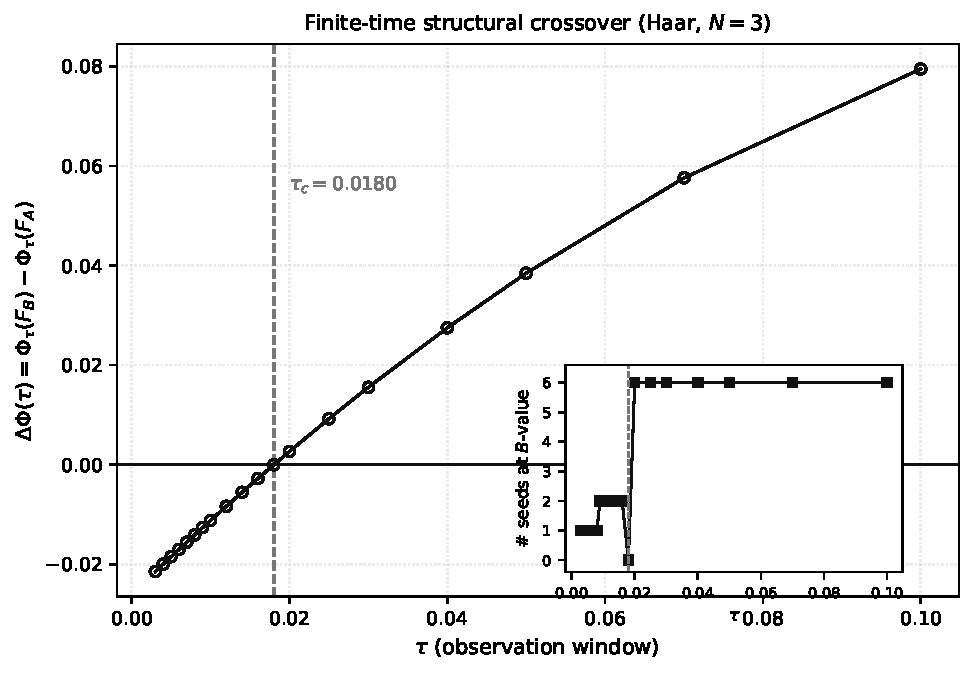
\includegraphics[keepaspectratio,alt={Figure 2: Finite-time structural crossover (Claim 4a, D3; Haar, N=3). \textbackslash Delta\textbackslash Phi(\textbackslash tau) = \textbackslash Phi\_\textbackslash tau(F\_B) - \textbackslash Phi\_\textbackslash tau(F\_A) at fixed representatives (main panel): the curve is smooth and monotone and crosses zero at the objective crossing \textbackslash tau\_c = 0.0180 (dashed vertical line); the crossover is defined by \textbackslash Delta\textbackslash Phi(\textbackslash tau\_c)=0, never by optimizer basin hops. Inset: number of optimizer seeds (of 6) sitting at the B-basin value flips from 0 to 6 between \textbackslash tau = 0.018 and \textbackslash tau = 0.02 --- the optimizer follows the objective crossing.}]{figures/fig2_crossover}}
\caption{Figure 2: Finite-time structural crossover (Claim 4a, D3; Haar,
\(N=3\)). \(\Delta\Phi(\tau) = \Phi_\tau(F_B) - \Phi_\tau(F_A)\) at
fixed representatives (main panel): the curve is smooth and monotone and
crosses zero at the objective crossing \(\tau_c = 0.0180\) (dashed
vertical line); the crossover is defined by \(\Delta\Phi(\tau_c)=0\),
never by optimizer basin hops. Inset: number of optimizer seeds (of 6)
sitting at the \(B\)-basin value flips from 0 to 6 between
\(\tau = 0.018\) and \(\tau = 0.02\) --- the optimizer follows the
objective crossing.}
\end{figure}

\emph{Transition nature.} The objective crossing is continuous (smooth
monotone \(\Delta\Phi\)), but the structural realization is
\textbf{first-order-like}: the best solution hops between distinct local
maxima (adjacent-\(\tau\) \(d_F\) jumps \(O(1)\) at \(\tau=0.02\) and
\(0.05\)) and reaches \(F_B\) exactly at \(\tau=0.1\) (\(d_F=0.000\)).
In a finite-dimensional system we use the language ``sharp structural
crossover / first-order-like basin transition'', not ``phase
transition''.

\emph{Methodological note.} Per-seed basin labels via \(d_F\) to fixed
representatives are \textbf{not meaningful} on the quotient (many
distinct local maxima sit \(\approx 0.87\) from \emph{both}
representatives); value-based classification (closeness to
\(\Phi_\tau(F_A)\) vs \(\Phi_\tau(F_B)\)) is the correct tool. The
crossover is defined by the objective crossing, which cleanly separates
optimizer basin hopping from the physical structural transition.

\emph{State dependence (D3-7).} The presence and location of the
crossover are state-dependent: ground and mixed show \textbf{no}
crossover up to \(\tau=1.0\) (\(d_F\) drift \(\le 0.12\),
\(\Delta\Phi \approx 0\)), while thermal has one with
\(\tau_c \in (0.3, 1.0)\) (\(d_F = 0.879\)). The precise statement is:
\emph{relational structure can depend systematically on the dynamical
observation scale, with the presence and location of crossovers being
state-dependent.}

\section{7. Claim 4b --- finite-size persistence
(D4)}\label{claim-4b-finite-size-persistence-d4}

\textbf{Claim 4b.} \emph{The structural crossover persists as the
Hilbert-space size increases:
\(\tau_c = 0.0180, 0.0206, 0.0224, 0.0217\) for \(N = 3\) (\(2|1\)),
\(N=4\) (\(2|2\)), \(N=4\) (\(1|3\)), \(N=5\) (\(2|3\), full quotient).
Within \(N=3\text{–}5\) this is an essentially size-independent
finite-size trend.}

\emph{Well-posedness vs \(N\) (D4-A; \(J_{\mathrm{dyn}}^{(0)}\) only).}

{\def\LTcaptype{none} % do not increment counter
\begin{longtable}[]{@{}
  >{\raggedright\arraybackslash}p{(\linewidth - 16\tabcolsep) * \real{0.1111}}
  >{\raggedright\arraybackslash}p{(\linewidth - 16\tabcolsep) * \real{0.1111}}
  >{\raggedright\arraybackslash}p{(\linewidth - 16\tabcolsep) * \real{0.1111}}
  >{\raggedright\arraybackslash}p{(\linewidth - 16\tabcolsep) * \real{0.1111}}
  >{\raggedright\arraybackslash}p{(\linewidth - 16\tabcolsep) * \real{0.1111}}
  >{\raggedright\arraybackslash}p{(\linewidth - 16\tabcolsep) * \real{0.1111}}
  >{\raggedright\arraybackslash}p{(\linewidth - 16\tabcolsep) * \real{0.1111}}
  >{\raggedright\arraybackslash}p{(\linewidth - 16\tabcolsep) * \real{0.1111}}
  >{\raggedright\arraybackslash}p{(\linewidth - 16\tabcolsep) * \real{0.1111}}@{}}
\toprule\noalign{}
\begin{minipage}[b]{\linewidth}\raggedright
\(N\)
\end{minipage} & \begin{minipage}[b]{\linewidth}\raggedright
cut
\end{minipage} & \begin{minipage}[b]{\linewidth}\raggedright
quotient
\end{minipage} & \begin{minipage}[b]{\linewidth}\raggedright
state
\end{minipage} & \begin{minipage}[b]{\linewidth}\raggedright
\(\Phi^*\)
\end{minipage} & \begin{minipage}[b]{\linewidth}\raggedright
std
\end{minipage} & \begin{minipage}[b]{\linewidth}\raggedright
\(\tilde I\)
\end{minipage} & \begin{minipage}[b]{\linewidth}\raggedright
min \(C_F^2\)
\end{minipage} & \begin{minipage}[b]{\linewidth}\raggedright
\(p_{\max}\)
\end{minipage} \\
\midrule\noalign{}
\endhead
\bottomrule\noalign{}
\endlastfoot
3 & \(2\|1\) & 45 (full) & ground & 1.8995 & 0.0007 & 1.000 & 0.500 &
0.51 \\
3 & \(2\|1\) & 45 (full) & haar & 1.8594 & 0.0090 & 0.982 & 0.487 &
0.58 \\
4 & \(2\|2\) & 225 (full) & ground & 3.6923 & 0.0008 & 0.999 & 0.749 &
0.27 \\
4 & \(2\|2\) & 225 (full) & haar & 3.7041 & 0.0008 & 0.997 & 0.748 &
0.28 \\
5 & \(2\|3\) & 945 (full) & ground & 3.6713 & 0.0006 & 1.000 & 0.750 &
0.26 \\
5 & \(2\|3\) & 945 (full) & haar & 3.6346 & 0.0022 & 0.998 & 0.749 &
0.28 \\
\end{longtable}
}

Here \(\tilde I = I/(2\log_2 d_{\min}) \in [0,1]\) is the mutual
information normalized by its maximum for a pure state across the cut.
Well-posedness (no denominator) holds at all sizes: min
\(C_F^2 \ge 0.49\), \(p_{\max} \le 0.58\), seed std \(\le 0.009\);
\(\tilde I \approx 0.98\text{–}
1.00\) --- the selected structures articulate near-maximal information.

\emph{Crossover persistence (D4-B; Haar primary; \(\Delta\Phi\) at fixed
reps).}

{\def\LTcaptype{none} % do not increment counter
\begin{longtable}[]{@{}lllll@{}}
\toprule\noalign{}
\(N\) & cut & quotient & \(d_F(F_A,F_B)\) & \(\tau_c\) \\
\midrule\noalign{}
\endhead
\bottomrule\noalign{}
\endlastfoot
3 & \(2\|1\) & 45 (full) & 0.886 & \textbf{0.0180} \\
4 & \(2\|2\) & 225 (full) & 0.968 & \textbf{0.0206} \\
4 & \(1\|3\) & 189 (full) & 0.994 & \textbf{0.0224} \\
5 & \(2\|3\) & 945 (full) & 0.319 & \textbf{0.0217} \\
\end{longtable}
}

The crossover exists at \(N=4,5\) with \(\Delta\Phi\) sign flips within
\(\tau \in [10^{-3}, 1]\) and genuinely distinct competing basins (Fig.
3). The N=4 balanced (\(2|2\)) vs asymmetric (\(1|3\)) control gives
nearly identical \(\tau_c\) (\(0.021\) vs \(0.022\)):
\textbf{bipartition shape has little effect at fixed size}, which
validates the \(N=5\) (asymmetric \(2|3\)) reading as a size effect
rather than a shape artifact. The \(N=5\) full-quotient closure confirms
persistence under full TPS optimization; the interesting contrast
\(d_F = 0.319\) (full) vs \(0.992\) (200-dim random subspace, see
Supplementary) shows the full quotient finds closer competing basins
while the crossing and timescale are unchanged.

\begin{figure}
\centering
\pandocbounded{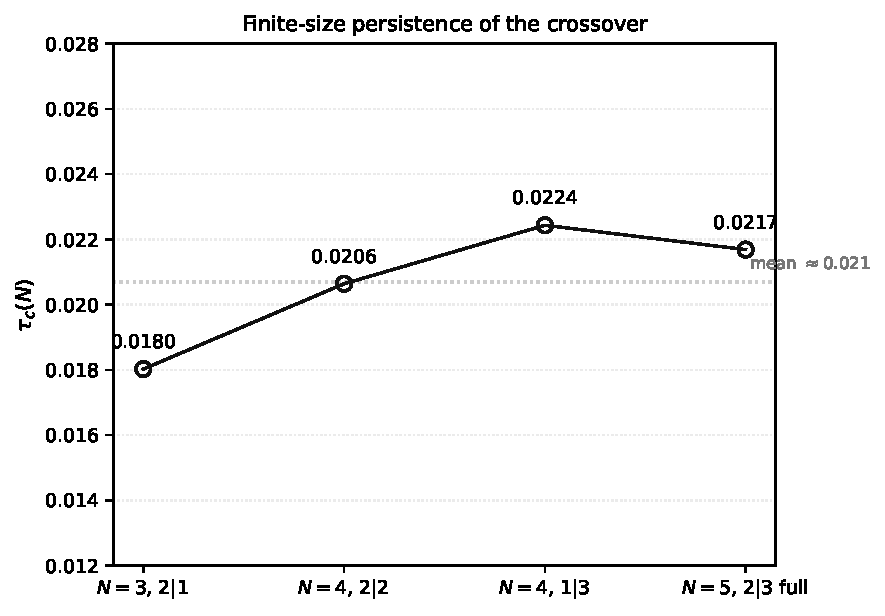
\includegraphics[keepaspectratio,alt={Figure 3: Finite-size persistence of the crossover (Claim 4b, D4). \textbackslash tau\_c(N) for N=3 (cut 2\textbar1, full 45-dim), N=4 (2\textbar2, full 225-dim), N=4 (1\textbar3, full 189-dim), N=5 (2\textbar3, full 945-dim): \textbackslash tau\_c = 0.0180, 0.0206, 0.0224, 0.0217. The crossover persists across Hilbert-space sizes with an essentially flat timescale (dotted line: mean \textbackslash approx 0.021) --- finite-size persistence, not a thermodynamic scaling law.}]{figures/fig3_tau_c_trend}}
\caption{Figure 3: Finite-size persistence of the crossover (Claim 4b,
D4). \(\tau_c(N)\) for \(N=3\) (cut \(2|1\), full 45-dim), \(N=4\)
(\(2|2\), full 225-dim), \(N=4\) (\(1|3\), full 189-dim), \(N=5\)
(\(2|3\), full 945-dim): \(\tau_c = 0.0180, 0.0206, 0.0224, 0.0217\).
The crossover persists across Hilbert-space sizes with an essentially
flat timescale (dotted line: mean \(\approx 0.021\)) --- finite-size
persistence, not a thermodynamic scaling law.}
\end{figure}

Scope: \(N = 3\text{–}5\) establishes \textbf{finite-size persistence /
finite-size trend} --- not a scaling law and not a thermodynamic limit.

\section{8. Claim 4c --- crossover mechanism (Phase
E)}\label{claim-4c-crossover-mechanism-phase-e}

\textbf{Claim 4c.} \emph{The crossover timescale is a derived quantity:
to first order in the finite-time expansion,}

\[\tau_c^{(1)} = -\frac{\Delta\Phi_0}{\Delta\Phi_1},\]

\emph{with \(\Delta\Phi_0 = \Phi_0(F_B) - \Phi_0(F_A)\) and
\(\Delta\Phi_1 =
\frac{d}{d\tau}\Delta\Phi(\tau)\big|_0\). It reproduces the measured
\(\tau_c\) within 5--11\%, and the quadratic correction within
0.0--0.5\%.}

\emph{Derivation.} Expanding
\(J_\tau(F) = J_0(F) + \tau J_1(F) + O(\tau^2)\), with \(I_F\)
independent of \(\tau\), gives
\(\Delta\Phi(\tau) = \Delta\Phi_0 + \tau\Delta\Phi_1 + \tau^2\Delta\Phi_2
+ \cdots\), hence the crossing \(\Delta\Phi(\tau_c)=0\) implies the
boxed formula to first order. The first-order coefficient is computed
both numerically (small-\(\tau\) slope) and analytically. With the fixed
Schmidt basis \(Q_F\),
\(C^2(\tau) = |Q_F U^\dagger e^{\tau L}\rho\, U|^2\) and
\(C^2(0) = |Q_F\rho_U|^2\), \(C^2{}'(0) = 2\mathrm{Re}\langle Q_F\rho_U,
Q_F Y_U\rangle\) with \(Y_U = U^\dagger L\rho_0 U\); the second
derivative is

\[C^2{}''(0) = 2|Q_F Y_U|^2 + 2\mathrm{Re}\langle Q_F\rho_U,
Q_F(U^\dagger L^2\rho_0 U)\rangle,\]

so \(J_1 = -C^2{}''(0)/4\).

\emph{Evidence (fixed reps from D3/D4; \(N=5\) uses the full-quotient
official value \(0.0217\)).}

{\def\LTcaptype{none} % do not increment counter
\begin{longtable}[]{@{}
  >{\raggedright\arraybackslash}p{(\linewidth - 14\tabcolsep) * \real{0.1250}}
  >{\raggedright\arraybackslash}p{(\linewidth - 14\tabcolsep) * \real{0.1250}}
  >{\raggedright\arraybackslash}p{(\linewidth - 14\tabcolsep) * \real{0.1250}}
  >{\raggedright\arraybackslash}p{(\linewidth - 14\tabcolsep) * \real{0.1250}}
  >{\raggedright\arraybackslash}p{(\linewidth - 14\tabcolsep) * \real{0.1250}}
  >{\raggedright\arraybackslash}p{(\linewidth - 14\tabcolsep) * \real{0.1250}}
  >{\raggedright\arraybackslash}p{(\linewidth - 14\tabcolsep) * \real{0.1250}}
  >{\raggedright\arraybackslash}p{(\linewidth - 14\tabcolsep) * \real{0.1250}}@{}}
\toprule\noalign{}
\begin{minipage}[b]{\linewidth}\raggedright
System
\end{minipage} & \begin{minipage}[b]{\linewidth}\raggedright
\(\Delta\Phi_0\)
\end{minipage} & \begin{minipage}[b]{\linewidth}\raggedright
\(\Delta\Phi_1\) (num / ana)
\end{minipage} & \begin{minipage}[b]{\linewidth}\raggedright
\(\tau_c^{(1)}\)
\end{minipage} & \begin{minipage}[b]{\linewidth}\raggedright
\(\tau_c^{(2)}\)
\end{minipage} & \begin{minipage}[b]{\linewidth}\raggedright
measured
\end{minipage} & \begin{minipage}[b]{\linewidth}\raggedright
err(1st)
\end{minipage} & \begin{minipage}[b]{\linewidth}\raggedright
err(2nd)
\end{minipage} \\
\midrule\noalign{}
\endhead
\bottomrule\noalign{}
\endlastfoot
\(N=3,\ 2\|1\) & −0.0260 & +1.521 / +1.526 & 0.0171 & 0.0180 & 0.0180 &
5.1\% & 0.1\% \\
\(N=4,\ 2\|2\) & −0.0099 & +0.526 / +0.528 & 0.0188 & 0.0206 & 0.0206 &
8.6\% & 0.0\% \\
\(N=4,\ 1\|3\) & −0.0339 & +1.633 / +1.639 & 0.0208 & 0.0224 & 0.0224 &
7.2\% & 0.2\% \\
\(N=5,\ 2\|3\) & −0.0219 & +1.130 / +1.136 & 0.0193 & 0.0216 & 0.0217 &
10.9\% & 0.5\% \\
\end{longtable}
}

\emph{Gates.} (E1) The expansion \(J_\tau = J_0 + \tau J_1 + O(\tau^2)\)
holds numerically:
\(|J_\tau - J_0 - \tau J_1^{\mathrm{ana}}| \le 2.4\times10^{-5}\) at
\(\tau=10^{-3}\), and the analytic \(J_1\) matches the numerical slope
in all four cases (Fig. 4). (E2) The crossover-generating sign structure
\(\Delta\Phi_0 < 0 < \Delta\Phi_1\) holds in all four cases: \(F_A\) is
instantaneously better, \(F_B\)'s advantage grows with \(\tau\). (E3)
First order within 5.1--10.9\% (\(\le 20\%\) tolerance). (E4) The
predicted flatness (spread \(0.195\)) matches the measured flat trend
(spread \(0.213\)): the size-independent \(\tau_c\) is explained by the
size-independent ratio \(-\Delta\Phi_0/\Delta\Phi_1\). (E5) The
quadratic correction improves systematically: mean relative error drops
from 7.96\% (first order) to 0.21\% (quadratic);
\(\tau_c^{(2)} = 0.0180, 0.0206,
0.0224, 0.0216\). (E6) Inter-basin objective competition (5--11\% error)
decisively outperforms the Liouvillian gap timescale (83--136× off; see
Sec. 9).

\begin{figure}
\centering
\pandocbounded{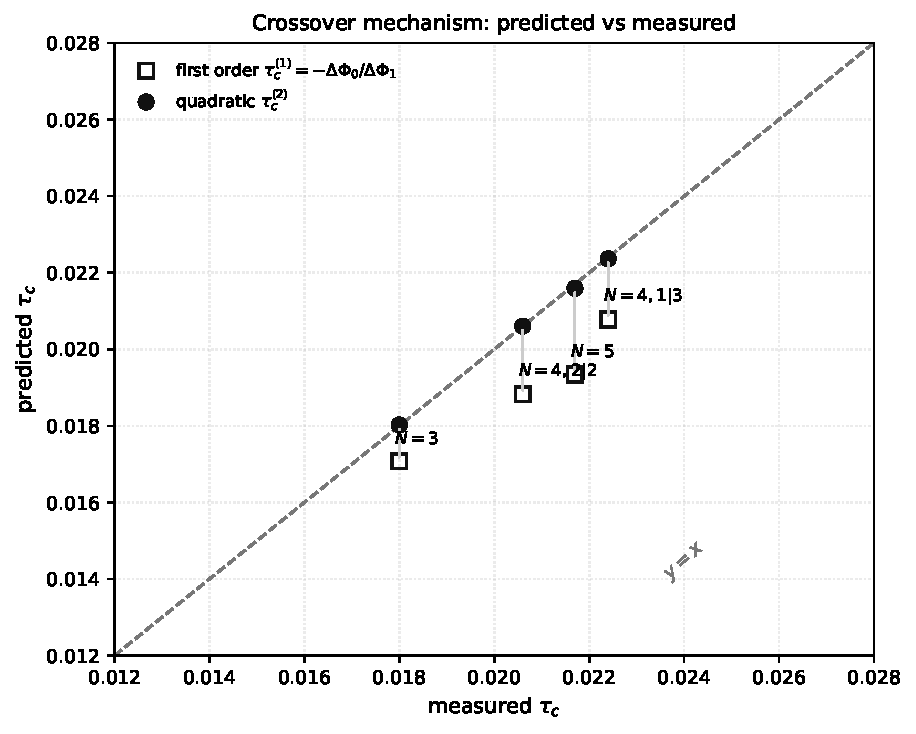
\includegraphics[keepaspectratio,alt={Figure 4: Crossover mechanism (Claim 4c, Phase E). Predicted \textbackslash tau\_c\^{}\{(1)\} = -\textbackslash Delta\textbackslash Phi\_0/\textbackslash Delta\textbackslash Phi\_1 (open squares) and quadratic \textbackslash tau\_c\^{}\{(2)\} (filled circles) vs the measured \textbackslash tau\_c for the four systems; the dashed diagonal is y = x. First order reproduces the measured values within 5.1--10.9\%; the quadratic correction places the predictions on the diagonal (0.0--0.5\% relative error) --- the crossover timescale is derived, not fitted.}]{figures/fig4_mechanism}}
\caption{Figure 4: Crossover mechanism (Claim 4c, Phase E). Predicted
\(\tau_c^{(1)} = -\Delta\Phi_0/\Delta\Phi_1\) (open squares) and
quadratic \(\tau_c^{(2)}\) (filled circles) vs the measured \(\tau_c\)
for the four systems; the dashed diagonal is \(y = x\). First order
reproduces the measured values within 5.1--10.9\%; the quadratic
correction places the predictions on the diagonal (0.0--0.5\% relative
error) --- the crossover timescale is derived, not fitted.}
\end{figure}

\section{9. Discussion}\label{discussion}

\subsection{9.1 The Liouvillian-gap hypothesis is
rejected}\label{the-liouvillian-gap-hypothesis-is-rejected}

A natural guess is that the crossover scale is set by the slowest
relaxation mode of the environment, \(\tau_L = \Delta_L^{-1}\) with
\(\Delta_L = \min_{\mu\ne 0}|\mathrm{Re}\,\mu|\) over the Liouvillian
spectrum. The data reject it:

\[\tau_c\Delta_L = 0.0119 \quad (N=3),\qquad
\frac{\tau_L}{\tau_c} \approx 83\text{–}136 \quad (N=3\text{–}5).\]

The measured \(\tau_c \approx 0.02\) is two orders of magnitude
\emph{shorter} than the Liouvillian gap timescale, and the ratio is
state-dependent (for thermal, with \(\tau_c \in (0.3, 1.0)\), it would
be \(\sim 0.2\text{–}0.66\)) --- not concentrated. The crossover scale
is therefore \textbf{not simply set by the global Liouvillian relaxation
time}. This negative result is kept as a constraint: any mechanistic
account of \(\tau_c\) must explain why it is so much shorter than
\(\tau_L\).

\subsection{9.2 The crossover scale as an objective
balance}\label{the-crossover-scale-as-an-objective-balance}

Claim 4c provides the positive account: \(\tau_c \approx
-\Delta\Phi_0/\Delta\Phi_1\) is the ratio of the instantaneous
disadvantage of basin \(B\) (\(\Delta\Phi_0 < 0\)) to the rate at which
\(B\)'s finite-window advantage grows (\(\Delta\Phi_1 > 0\)). The
structure that is worse at \(t=0\) wins once the window is long enough.
This is a statement about the geometry of the objective landscape, not
about the relaxation spectrum of \(L\); it explains both the magnitude
(\(\tau_c \sim |\Delta\Phi_0| /
|\Delta\Phi_1| \approx 0.02\)) and the flatness across \(N\) (both
\(\Delta\Phi_0\) and \(\Delta\Phi_1\) are size-insensitive in the tested
range).

\subsection{9.3 Limitations and scope}\label{limitations-and-scope}

\begin{itemize}
\tightlist
\item
  \textbf{Finite dimension, finite size}: \(N \le 5\), four systems;
  ``finite-size persistence / trend'', not a scaling law or
  thermodynamic limit. All statements use ``sharp structural crossover /
  first-order-like basin transition'', not ``phase transition''.
\item
  \textbf{State dependence}: the crossover is present for Haar (and
  thermal at larger \(\tau\)), absent for ground and mixed up to
  \(\tau=1\). The precise claim is that relational structure \emph{can}
  depend on the observation scale, with the presence and location of
  crossovers state-dependent.
\item
  \textbf{Protocol reductions}: the \(N=5\) full-quotient run used 2
  seeds × 100 steps (documented; std \(2\times10^{-4}\)). A 200-dim
  random-subspace search at \(N=5\) is retained in the Supplementary as
  restricted-domain history (it gave \(\tau_c = 0.0173\), a slight
  underestimate).
\item
  \textbf{Optimizer}: finite-difference Adam on the quotient; the
  crossover analysis itself is objective-level (fixed representatives)
  and does not depend on optimizer convergence details.
\item
  \textbf{Separation of concerns}: the frozen specification (Spec v2.2)
  is not modified by this paper's evidence; the verification trail is
  documented in the Validation Addendum.
\end{itemize}

\subsection{9.4 Implications}\label{implications}

The arc falsified → replaced → survived has a methodological moral for
variational structure selection: objectives must be checked for
denominator singularities on the \emph{unrestricted} domain, and the
finite observation window is not a harmless technicality --- it changes
the selected structure qualitatively through genuine basin competition.
For REM, the dynamical-scale dependence of \(F^*\) is not a defect but a
feature: the same state admits different optimal relational structures
depending on the timescale over which stability is assessed, with a
characteristic scale set by the competition between basins.

\section{10. Conclusion}\label{conclusion}

We have established four claims numerically for the variational
tensor-product selection program of the Relational Emergence Model:

\begin{enumerate}
\def\labelenumi{\arabic{enumi}.}
\tightlist
\item
  the normalized local decay rate is \textbf{singular} on the
  unrestricted quotient and is prohibited as a global objective (D2.1);
\item
  the unnormalized canonical functional \(J_{\mathrm{dyn}}^{(0)}\) is
  \textbf{well-posed} --- singularity, product collapse, and seed
  instability disappear (D2.2);
\item
  the selected structure \(F^* = F^*(\rho, L, \lambda)\)
  \textbf{responds} to Hamiltonian and state (D1-R, D2-R);
\item
  a \textbf{finite-time structural crossover} exists between competing
  basins, persists across \(N = 3\text{–}5\) with
  \(\tau_c = 0.0180, 0.0206, 0.0224,
  0.0217\), and its characteristic scale is \textbf{derived} from the
  leading terms of the finite-time expansion,
  \(\tau_c \approx -\Delta\Phi_0/
  \Delta\Phi_1\) (5--11\% first order, 0.0--0.5\% with the quadratic
  correction) --- an inter-basin objective balance, not the Liouvillian
  relaxation time.
\end{enumerate}

The central contribution is the research arc itself: a canonical
functional was falsified mid-course, its replacement survived a battery
of tests, and the emergent phenomenon (structural crossover) was both
characterized and explained. The next steps are the publication pipeline
(figures, QC, independent review) and the extension of the mechanism
analysis to the thermal crossover and to larger systems where a genuine
scaling question becomes accessible.

\section{Supplementary --- restricted-domain history and additional
brackets}\label{supplementary-restricted-domain-history-and-additional-brackets}

\textbf{S1. \(N=5\) 200-dim random-subspace search.} Before the
full-quotient closure, the \(N=5\) crossover was measured on a 200-dim
random horizontal subspace of the 945-dim quotient (21\% of the
dimension; the repo's established \(n_{\mathrm{params}}\) heuristic for
large \(N\)). It gave \(\tau_c = 0.0173\) with \(d_F(F_A,F_B) = 0.992\).
The full-quotient closure (2 seeds × 100 steps) gives the official value
\(\tau_c(5) = 0.0217\) with \(d_F = 0.319\). The subspace value is
retained here as restricted-domain history only; the main text uses the
full-quotient value.

\begin{figure}
\centering
\pandocbounded{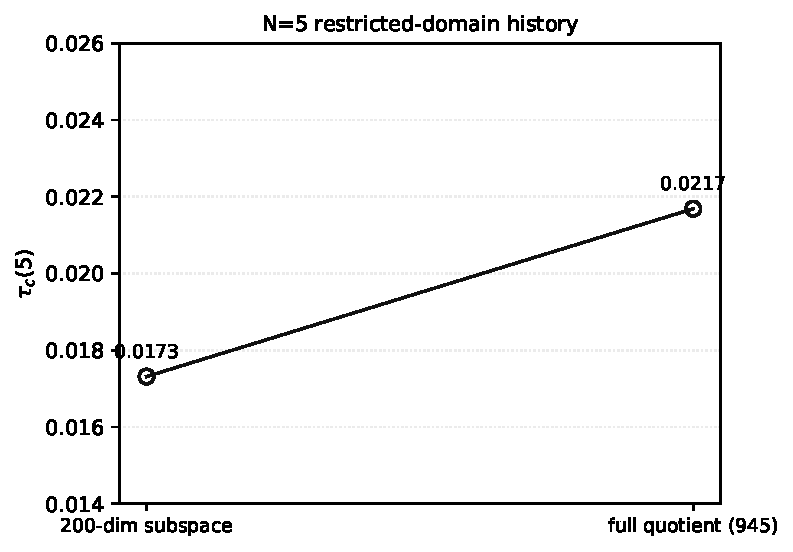
\includegraphics[keepaspectratio,alt={Supplementary Figure S1: N=5 restricted-domain history. The 200-dim random-subspace search gave \textbackslash tau\_c = 0.0173; the full-quotient closure (945-dim) gives the official value \textbackslash tau\_c = 0.0217 used in the main text.}]{figures/figS1_subspace}}
\caption{Supplementary Figure S1: N=5 restricted-domain history. The
200-dim random-subspace search gave \(\tau_c = 0.0173\); the
full-quotient closure (945-dim) gives the official value
\(\tau_c = 0.0217\) used in the main text.}
\end{figure}

\textbf{S2. Thermal crossover bracket.} For the thermal state,
\(\Delta\Phi(\tau)\) crosses zero between \(\tau = 0.3\) and
\(\tau = 1.0\): \(\Delta\Phi = -0.0109\) (0.2), \(-0.0046\) (0.3),
\(+0.0011\) (1.0), with \(d_F(F_A,F_B) = 0.879\). The precise location
is a target for future work (Phase E extension).

\textbf{S3. Protocol table.} Frozen conditions: asymmetric XY chain
\(J_1=1.5, J_i=0.6\), \(h=0.2\); dephasing \(\gamma=(0.5,1,2)\)
periodic; \(\lambda=0.2\); Adam lr \(10^{-2}\); seeds \(20260813\)
(D-series) / \(20260812\) (D1-series); steps 200 (\(N=3\)), 100
(\(N\ge4\)); seeds 6 (\(N=3\)), 4 (\(N=4,5\) subspace), 2 (\(N=5\) full
closure). All scripts, JSON outputs, and commits are listed in the Phase
D Validation Report §9.

\section{Data and code availability}\label{data-and-code-availability}

All scripts and outputs live in the public repository
\texttt{github.com/malko73/rem} (branch \texttt{open}): D-series scripts
under \texttt{analysis/}, results under \texttt{analysis\_output/},
frozen specification \texttt{REM\_spec\_v2\_2.md} with pandoc-generated
\texttt{papers/REM\_spec\_v2\_2.tex}, and this paper under
\texttt{papers/REM\_paper\_v0\_1.md}. Test suite: 74 passed + 1 xfailed
(plain \texttt{pytest}).

\end{document}
